\documentclass[main.tex]{subfiles}
\begin{document}

\chapter{The SD-433 dataset}
\label{chap:sd433_dataset}
\selectlanguage{english}

% The measurement of the energy spectrum of Cosmic Rays provides challenge in many different aspects.
% Since it's a key measurement with important astrophysical implications, obtaining the cleanest dataset possible is of utmost importance.
% In this chapter, the elements required to ensure the proper reconstruction are presented.
% In \cref{sec:triggers} the hierarchical set of triggers that build an event, from a station level to a physical level are described.
% Together with this in \cref{sec:efficiency}, the trigger efficiency is presented in order to determine the energy threshold when the exposure calculation becomes purely geometrical.
% Finally the array stability is discussed in \cref{sec:stability} together with the history of the array in order to properly determine the exposure to be used in the spectrum measurement.

% The measurement of the cosmic-ray energy spectrum poses several experimental challenges.
% Since this observable has important astrophysical implications, the construction of a clean and well-understood dataset is essential.
% This requires not only a reliable event reconstruction but also a careful characterization of the detector response, the trigger efficiency, and the stability of the array over time.

% This chapter introduces the main elements that define the dataset used in this work.
% It begins with the hierarchical trigger chain, from the local station triggers to the selection of physical events, described in \cref{sec:triggers}.
% Then, \cref{sec:efficiency} addresses the trigger efficiency and establishes the energy threshold above which the exposure can be treated as purely geometrical.
% The discussion closes with the stability and operational history of the array in \cref{sec:stability}, which provides the basis for the exposure calculation used in the spectrum measurement.

% \section{The Surface Detector Triggers}
% \label{sec:triggers}

% To discriminate signals produced by an \gls{eas}, initiated by the interaction of a primary \gls{cr} in the atmosphere, a set of triggers is implemented.
% \Cref{fig:t1t2t3} summarizes the station-level T1 and T2 triggers, as well as the array-level T3 trigger.

% Originally, two T1 trigger modes were deployed: the \gls{th}-T1 (threshold) and the \gls{tot}.
% In the first case, a signal larger than $1.75\,I_{\text{VEM}}^{\text{peak}}$ is required in each of the three \gls{pmt}s.
% This trigger is designed to select larger signals that are not necessarily spread over time and is particularly sensitive to inclined showers with a stronger muonic component.

% The \gls{tot} trigger requires a signal above $0.2\,I_{\text{VEM}}^{\text{peak}}$ in at least two \gls{pmt}s for at least 13 time bins within a \SI{3}{\micro\s} window.
% This trigger is designed for moderately inclined, lower-energy showers, in which the particles arriving at the \gls{wcd} are spread over time, as well as for higher-energy showers with distant cores.
% A detailed discussion of the original triggers is given in Ref.~\cite{PierreAuger:2011TriggerAndApperture}.

% In 2014, two new trigger modes were introduced.
% These triggers target lower-energy showers detected by the denser \sd{433} and \sd{750} arrays and are more sensitive to the electromagnetic component of the shower.
% The \gls{totd} trigger is based on the idea that signals with a significant electromagnetic component have a shape similar to a \gls{tot} trace, with a pronounced rise followed by an exponential decay.
% After deconvolution, the expected signal becomes approximately flat, although Poissonian fluctuations are allowed.
% The \gls{tot} requirement is then applied to the deconvoluted trace.

% The \gls{mops} trigger is independent of the \gls{vem} calibration and is based on the expected signal produced by multiple electromagnetic particles spread over time.
% It counts the number of instances within a \SI{3}{\micro\s} sliding window in which an increase in signal amplitude is observed in consecutive bins, that is, a positive step.
% This positive step must be larger than the typical noise level and smaller than the amplitude expected from a vertical muon.
% If more than four such positive-step instances are found, the \gls{mops} trigger is issued.

% \begin{figure}
%     \centering
%     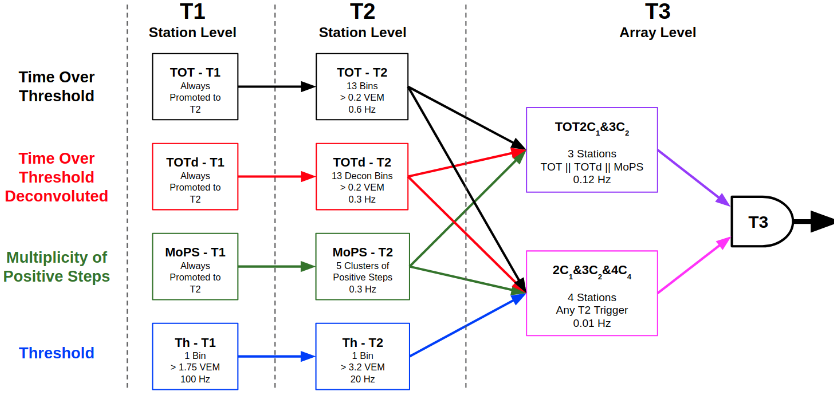
\includegraphics[width=\linewidth]{figures/chapter_dataset/provisory_t1t2t3.png}
%     \caption{Summary of the T1, T2 and T3 level triggers, thir requirements and average frequency. The \gls{tot}, \gls{totd} and \gls{mops} are automatically promoted to T2.}
%     \label{fig:t1t2t3}
% \end{figure}

% The \gls{tot}, \gls{totd} and \gls{mops} triggers are automatically promoted to the next level station trigger, T2.
% The \gls{th}-T1 trigger is requird to have a signal higher than  $3.2\,I_{\text{VEM}}^{\text{peak}}$ to be promoted to the T2 level.
% With the T2 the station level trigger frequency is reduced to ~\SI{20}{\Hz}, which is compatible with the bandwidth of the communication system.
% The \gls{cdas} analyzes the trigger kind and timestamp to find temporal and spatial correlation between  triggered stations.
% To form the next trigger level, the T3, two possible configurations are allowed.
% The central detector should have a \gls{tot} and be surrounded
% Once a T3 is formed, all traces from the detectors with a T2 level trigger and T1 for stations with a T1 closer than \SI{30}{\micro\s} of the T3 are stored in CDAS.

% Preliminary draft.
% TODO: Revisit the chapter roadmap once the full chapter is assembled.

The measurement of the cosmic-ray energy spectrum poses several experimental challenges.
Since this observable carries important astrophysical information, the construction of a clean and well-understood dataset is essential.
This requires not only a reliable event reconstruction, but also a careful characterization of the detector response, the trigger hierarchy, and the stability of the array over time.

This chapter introduces the main elements that define the dataset used in this work.
The \sd{433} is a compact array of 19 surface-detector stations arranged on a triangular grid with a spacing of \SI{433}{\m}, nested within the \sd{750} array to extend the energy-spectrum measurement toward lower energies~\cite{BrichettoOrquera:2023}.
It begins with the hierarchical trigger chain, from the local station triggers to the selection of physical events, described in \cref{sec:triggers}.
\cref{sec:efficiency} addresses the trigger efficiency and establishes the energy threshold above which the exposure can be treated as purely geometrical.
The discussion closes with the stability and operational history of the array in \cref{sec:stability}, which provides the basis for the exposure calculation in \cref{sec:exposure} used in the spectrum measurement.

\section{The Surface Detector Triggers}
\label{sec:triggers}

To discriminate signals produced by an \gls{eas}, initiated by the interaction of a primary \gls{cr} in the atmosphere, the surface detector uses a hierarchical trigger system.
This hierarchy begins at the level of individual stations and continues up to the selection of physical events and quality requirements at the array level.
A schematic summary of the trigger chain is shown in \cref{fig:t1t2t3}.

Originally, two T1 trigger modes were implemented at the station level: \gls{th}-T1, and \gls{tot}.
The \gls{th}-T1 trigger requires a signal larger than $1.75\,I_{\text{VEM}}^{\text{peak}}$ in each of the three \gls{pmt}s.
This trigger is designed to select large signals that are not necessarily spread in time and is particularly sensitive to inclined showers with a stronger muonic component.

The \gls{tot} trigger requires that at least 13 bins within a sliding window of \SI{3}{\micro\s} exceed $0.2\,I_{\text{VEM}}^{\text{peak}}$ in coincidence in at least two \gls{pmt}s.
This trigger is designed to select sequences of smaller signals spread over time, as expected from the electromagnetic component of the shower.
It is therefore well suited to lower-energy showers and to events in which the detector is far from the shower core.

In 2014, two additional station-level trigger modes were introduced.
These triggers were designed to improve sensitivity to the electromagnetic component of the shower and to extend the energy range over which the array can detect events.

The first of these triggers is the \gls{totd} trigger.
Traces with a significant electromagnetic component resemble a \gls{tot} signal, with a fast rise followed by an exponential decay.
Deconvolution removes this characteristic exponential tail from the recorded trace.
The resulting signal is approximately flat while preserving the fluctuations associated with particle counting, and the \gls{tot} requirement is then applied.

The second additional trigger is the \gls{mops} trigger.
This trigger is independent of the \gls{vem} calibration and is based on the signal pattern expected from multiple low-amplitude particles arriving over an extended time interval.
It counts the number of positive steps within a \SI{3}{\micro\s} sliding window, where a positive step is defined as an increase in signal amplitude in consecutive bins.
To be counted, the step must be larger than the typical noise level and smaller than the amplitude expected from a vertical muon.
If more than four such positive-step instances are found, a \gls{mops} trigger is issued.
The \gls{mops} and \gls{mops} triggers are collectively referred as the Gen. II triggers.

\begin{figure}
    \centering
    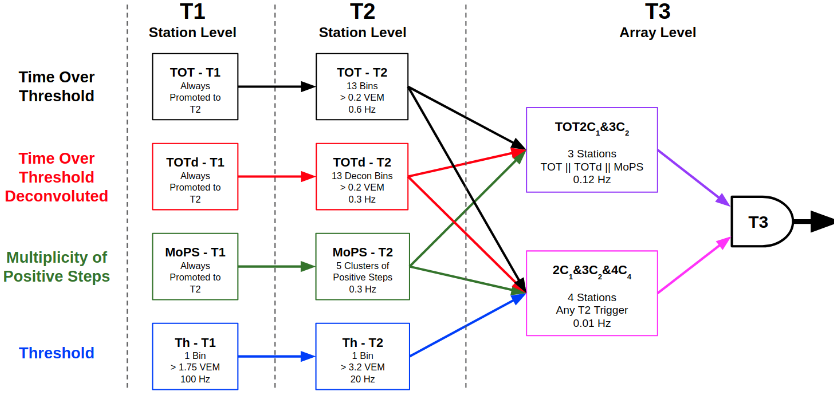
\includegraphics[width=\linewidth]{figures/chapter_dataset/provisory_t1t2t3.png}
    \caption{Summary of the T1, T2, and T3 trigger levels, their requirements, and their typical rates.
    The \gls{tot}, \gls{totd}, and \gls{mops} triggers are automatically promoted to the T2 level.}
    \label{fig:t1t2t3}
\end{figure}

The second trigger level, T2, is applied locally at each station to reduce the trigger rate to a value compatible with the bandwidth of the communication system.
All \gls{tot}, \gls{totd}, and \gls{mops} triggers are automatically promoted to T2.
By contrast, a \gls{th}-T1 trigger is promoted to T2 only if the signal exceeds a higher threshold of $3.2\,I_{\text{VEM}}^{\text{peak}}$ in coincidence in the three \gls{pmt}s.
At this stage, the trigger rate is reduced to about \SI{20}{\Hz} per station.

The T2 information, namely the trigger type and time stamp, is then sent to the \gls{cdas}, where array-level triggers are formed from spatial and temporal coincidences among stations.
This defines the third trigger level, T3, which initiates the data acquisition for the event.
Once a T3 is issued, the \gls{fadc} traces from all stations with a T2 trigger are sent to \gls{cdas}, together with those from stations that raised a T1, provided that their trigger time lies within \SI{30}{\micro\s} of the T3 timestamp.

\begin{figure}
    \centering
    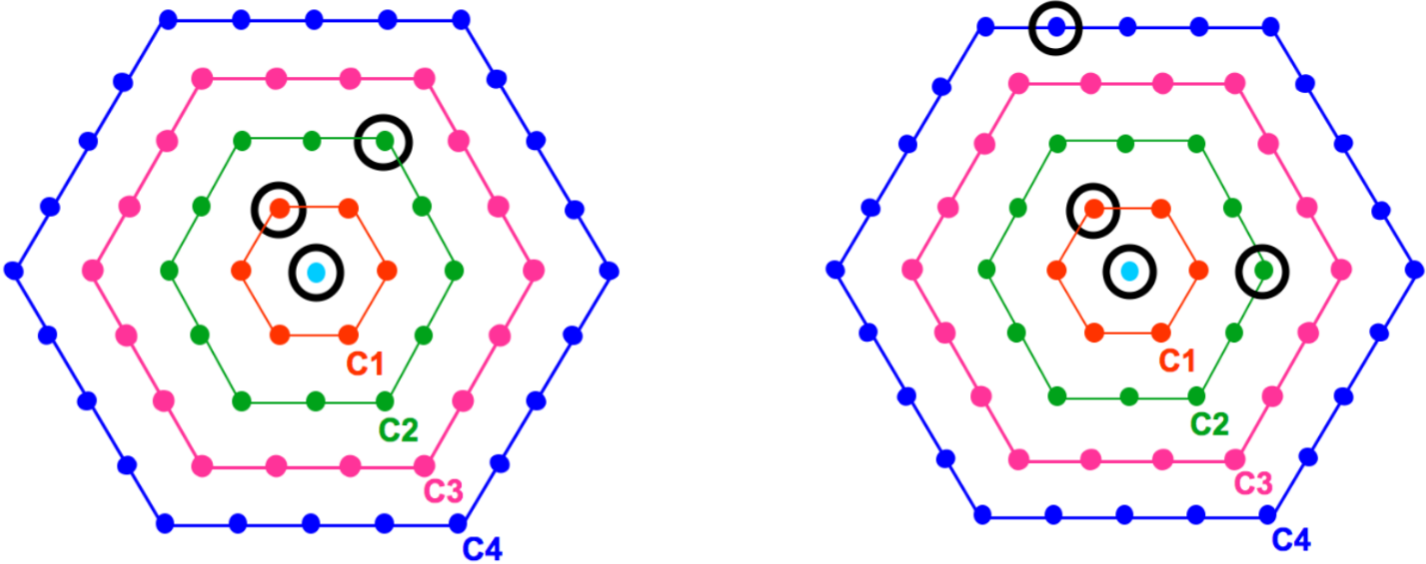
\includegraphics[width=\linewidth]{figures/chapter_dataset/provisory_t3.png}
    \caption{Examples of the two T3 triggering modes.
    Left: the three-fold configuration \textit{ToT2C1\&3C2}.
    Right: the four-fold configuration \textit{2C1\&3C2\&4C4}.
    Figure adapted from Fig.~2.14 of Ref.~\cite{Silli:2021:Thesis}.}
    \label{fig:t3}
\end{figure}

The search for temporal and spatial groupings is conducted using two types of T3 algorithms.
Both of them look for T2-triggered stations in a compact configuration.
The compactness is described by the number of crowns over which the triggered stations are spread.
A crown is a way of counting hexagons outward from a central station.

The first configuration, \textit{ToT2C1\&3C2}, requires a coincidence of at least three nearby stations passing any combination of \gls{tot}, \gls{totd}, and \gls{mops} triggers.
These stations must be in a compact pattern, such that one station has another one in the first crown and a third one in the second crown.
Since the \gls{tot} trigger has a very low background rate, this T3 mode has a low contamination and is highly efficient for showers with zenith angle below \SI{60}{\degree}.

The second T3 configuration, denoted \textit{2C1\&3C2\&4C4}, is more permissive.
It requires a four-fold coincidence of T2 stations, independently of their trigger type.
In this case, one triggered station must have another in the first crown, a third one in the second crown, and the fourth may be as far as the fourth crown.
This configuration is particularly relevant for more inclined showers, whose triggered stations can be spread over a wider area on the ground.

The T1, T2, and T3 selection are performed online and the data is stored to be reconstructed later, where the next two trigger levels are applied.
The physical trigger, T4,is designed to reject accidental coincidences and retain physically originated showers.
For vertical showers, two T4 criteria are used.

The first T4 criterion, denoted \textit{3ToT}, originally required three nearby stations having a \gls{tot} trigger in a non-aligned pattern, but was later updated to also include combinations of the \gls{totd} and \gls{mops} triggers.
In addition, the trigger times of the three stations must be compatible with a plane shower front moving at the speed of light.

The second T4 criterion, denoted \textit{4C1}, requires four nearby triggered stations without imposing any condition on the trigger type.
As in the 3ToT case, their times must be compatible with a plane shower front moving at the speed of light.
This criterion complements the 3ToT selection and improves the efficiency for events that are not selected by the more restrictive \gls{tot}-based condition.

To ensure reliable reconstruction, the 6T5 fiducial quality trigger requires the station with the highest signal to be surrounded by six active neighbouring stations.
This defines a regular hexagonal fiducial region containing the shower-core positions for which the highest-signal station is the closest detector, while excluding events near the boundary of the active array.
For a station spacing $d=\SI{433}{\m}$, the area of this hexagon is
\begin{align}
    S_{\mathrm{hex}}
    =\frac{\sqrt{3}}{2}d^2
    =\SI{0.162}{\km\squared}.
    \label{eq:6T5_area}
\end{align}

The event sample used in this work therefore consists of physical events selected by the T4 trigger that also satisfy the 6T5 fiducial requirement.

\section{Trigger Efficiency}
\label{sec:efficiency}

In order to calculate the exposure from the purely geometrical aperture of the array, it is necessary to establish an energy threshold above which the detector can be treated as fully efficient.
Below this threshold, the probability of detecting and reconstructing a shower depends on the primary energy and arrival direction, and the exposure can no longer be calculated from the geometry alone.
The spectrum measurement is therefore restricted to an energy range in which the array can be treated as fully efficient~\cite{PierreAuger:2010:TriggerAperture}.
The efficiency parameterization is nevertheless included in the detector response used in the forward-folding procedure to account for a residual detector influence near the threshold.

The efficiency of the \sd{433} array was studied in detail in Ref.~\cite{GAP:Rodriguez:2024:Efficiency}, using simulated showers and validating the results with measured data.
For this purpose, CORSIKA simulations were performed with EPOS-LHC~\cite{Pierog:2015:EPOSLHC} as the high-energy hadronic-interaction model and FLUKA~\cite{Battistoni:2008:FLUKA} at lower energies.
Seven primary mass groups, ranging from proton to iron, were simulated and reconstructed using the \sd{433} array.
Additionally, a mixed-composition result was estimated using the \gls{gsf} mix~\cite{Dembinski:2017:GSF}.
The study considers the probability that a shower with a given energy and zenith angle is successfully reconstructed by the array, after requiring the 6T5 condition and including the contribution of the \gls{totd} and \gls{mops} station triggers.
The efficiency is defined as the ratio of the number of simulated events successfully reconstructed by the \sd{433} to the total number of simulated events in the corresponding energy interval.
The simulation-based efficiency is transformed to the \sd{433} energy scale using the attenuation and calibration chain adopted for data~\cite{GAP:Rodriguez:2024:Efficiency}.

Efficiency studies of the \sd{433} are customarily restricted to events with $\theta<45^\circ$, since the quality of the standard geometry reconstruction degrades at larger zenith angles~\cite{GAP:Rodriguez:2024:Efficiency}.
In this work, the more conservative selection $\theta<40^\circ$ is adopted to match the zenith-angle range used for the \sd{750}~\cite{PierreAuger:2021:InfillSpectrum}.

The resulting efficiency in the \sd{433} energy scale is determined with an unbinned likelihood fit, considering if each simulated shower triggers the array or not.
The corresponding efficiency estimators and fits are shown in \cref{fig:sd433_efficiency_curve} for the \gls{gsf} mix, together with proton and iron as extreme cases.
For events with zenith angles $\theta<40^\circ$, the efficiency for the \gls{gsf} mix is parameterized as
\begin{align}
\epsilon(E) = \Phi \left( a_0 + a_1 \lg\left(\frac{E}{10^{17}\,\mathrm{eV}}\right) \right),
\label{eq:efficiency}
\end{align}
where $\Phi$ is the cumulative distribution function of the standard normal distribution, $E$ is the primary energy in the \sd{433} energy scale, $a_0$ determines the energy of the efficiency transition, and $a_1$ governs its steepness.
The fitted parameters for the \gls{gsf} mix are $a_0 = 4.21 \pm 0.03$ and $a_1 = 5.50 \pm 0.04$.
This parameterization will later be used in the forward-folding procedure described in \cref{chapter:SD433_Spectrum}.

Below full efficiency, the efficiency for proton showers is higher than that for iron showers.
This difference is linked to the deeper development of lighter-primary showers combined with the enhanced sensitivity of the second-generation triggers to the electromagnetic component of the shower~\cite{GAP:Rodriguez:2024:Efficiency}.
For proton, iron, and the \gls{gsf} mix, the first energy bin with an efficiency above $97\%$ begins at $\lg(E/\mathrm{eV})=16.7$.
This simulation-based result motivates the data-driven validations described below, which support the more conservative threshold of $\lg(E/\mathrm{eV})=16.8$ adopted for the spectrum measurement.
\begin{figure}
    \centering
    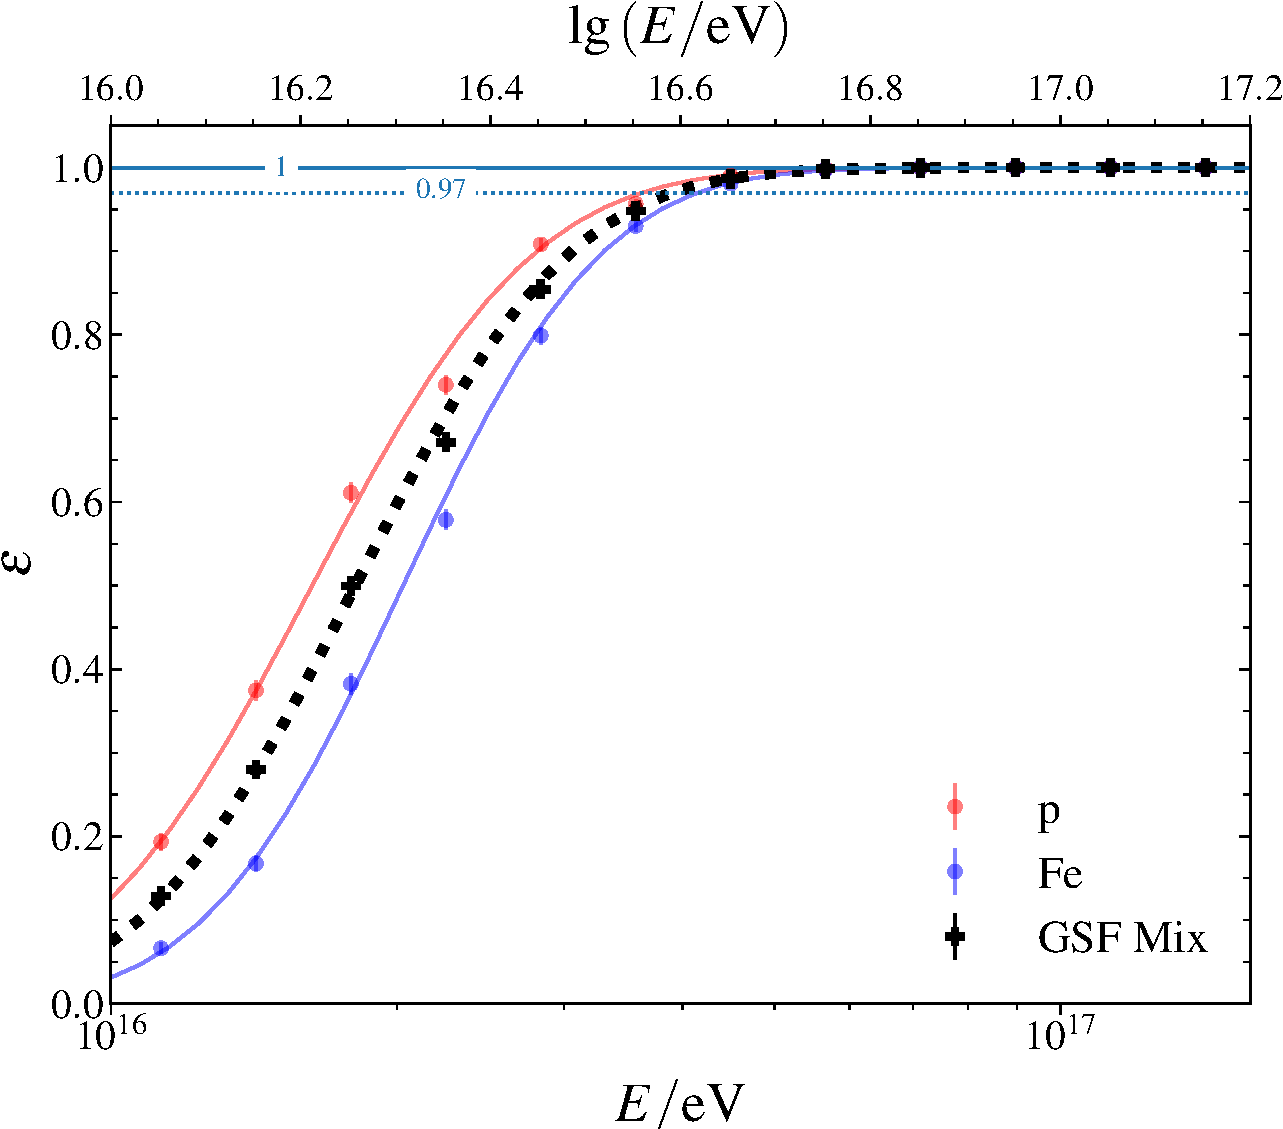
\includegraphics[width=0.5\linewidth]{figures/chapter_dataset/new_eff_SD433_scale-1-2.pdf}
    \caption{Efficiency curves as a function of the logarithm of the \sd{433} energy.
    Markers correspond to binned estimates of $\epsilon(E)$ obtained by dividing the number of triggered simulated showers by the total number of triggered and non-triggered simulated showers, while the lines show the unbinned fits.
    The inset highlights the region near full efficiency.
    Figure adapted from Fig.~7 of Ref.~\cite{GAP:Rodriguez:2024:Efficiency}.}
    \label{fig:sd433_efficiency_curve}
\end{figure}

The simulation-based efficiency result was cross-checked using two tests applied to reconstructed data.
These tests are dependent of the core and energy reconstruction procedures, since both require reconstructed event observables and calibrated energies.
Nevertheless, they probe two distinct signatures expected above full efficiency: the uniformity of the arrival directions in $\sin^2\theta$ and the uniform distribution of reconstructed shower cores within the fiducial 6T5 area.
Together, they provide data-driven validation of the threshold inferred from simulations.

The first data-driven validation tests the isotropy of the arrival directions above different energy thresholds, following Ref.~\cite{GAP:Rodriguez:2024:Efficiency}.
For isotropic arrival directions, the distribution in $\sin^2\theta$ is expected to be uniform up to the maximum zenith angle considered.
For each energy threshold, the cumulative distribution of $\sin^2\theta$ was compared with the uniform expectation using the Anderson--Darling test statistic, which gives greater weight to deviations near the tails of the distribution.
The reference distribution of the test statistic was generated from pseudo-experiments uniformly distributed in $\sin^2\theta$, and the $p$-value was calculated as the fraction of simulated statistics larger than the value observed in data.

The test gives numerical $p$-values of $0$, $0.008$, and $0.357$ for minimum-energy thresholds of $\lg(E/\mathrm{eV})=16.7$, $16.8$, and $16.9$, respectively.
Using $p<0.005$ as the rejection criterion, the isotropic hypothesis cannot be rejected for events with $\lg(E/\mathrm{eV})\geq16.8$.
This supports the choice of $\lg(E/\mathrm{eV})=16.8$ as a conservative threshold above which the array can be treated as fully efficient.

As a second validation, the spatial distribution of the reconstructed shower cores was examined using events with $\theta<40^\circ$.
Once the detector is fully efficient, an isotropic flux is expected to produce a uniform distribution of shower cores within the fiducial 6T5 area.
To combine the equivalent regions associated with different stations, the position of the station with the largest signal is subtracted from the reconstructed core position, folding all events into a single hexagon.

The resulting core positions are grouped using hexagonal bins with a characteristic size of approximately \SI{28}{\m}.
This choice preserves the symmetry of the detector and gives a spatial scale comparable to the core-position resolution, which is approximately \SI{20}{\m} in this energy range~\cite{GAP:Gonzalez:2020:Geometry}.
Bins adjacent to the boundary of the fiducial hexagon are excluded because fluctuations in the reconstructed core position can cause events near the edge to migrate across the boundary and distort the measured occupancy, causing border effects.

\Cref{fig:sd433_core_maps} shows the standardized deviation of the occupancy of each accepted bin from the mean occupancy,
\begin{align}
    \Delta n_i = \frac{n_i-\bar{n}}{\sigma_n},
\end{align}
where $n_i$ is the number of reconstructed cores in bin $i$, $\bar{n}$ is the mean occupancy of the accepted bins, and $\sigma_n$ is the standard deviation of their occupancies.

Without a minimum-energy requirement, the maps exhibit localized overdensities associated with reconstruction artifacts below full efficiency.
These structures become less pronounced as the minimum energy increases and the core reconstruction improves.
At $\lg(E/\mathrm{eV})=16.7$, an overdensity remains around the central station, consistent with reconstructed core positions being preferentially drawn toward the station with the largest signal.
This feature is no longer apparent from $\lg(E/\mathrm{eV})=16.8$ onward, for which the cores populate the fiducial area more uniformly.

\begin{figure}

    \centering
    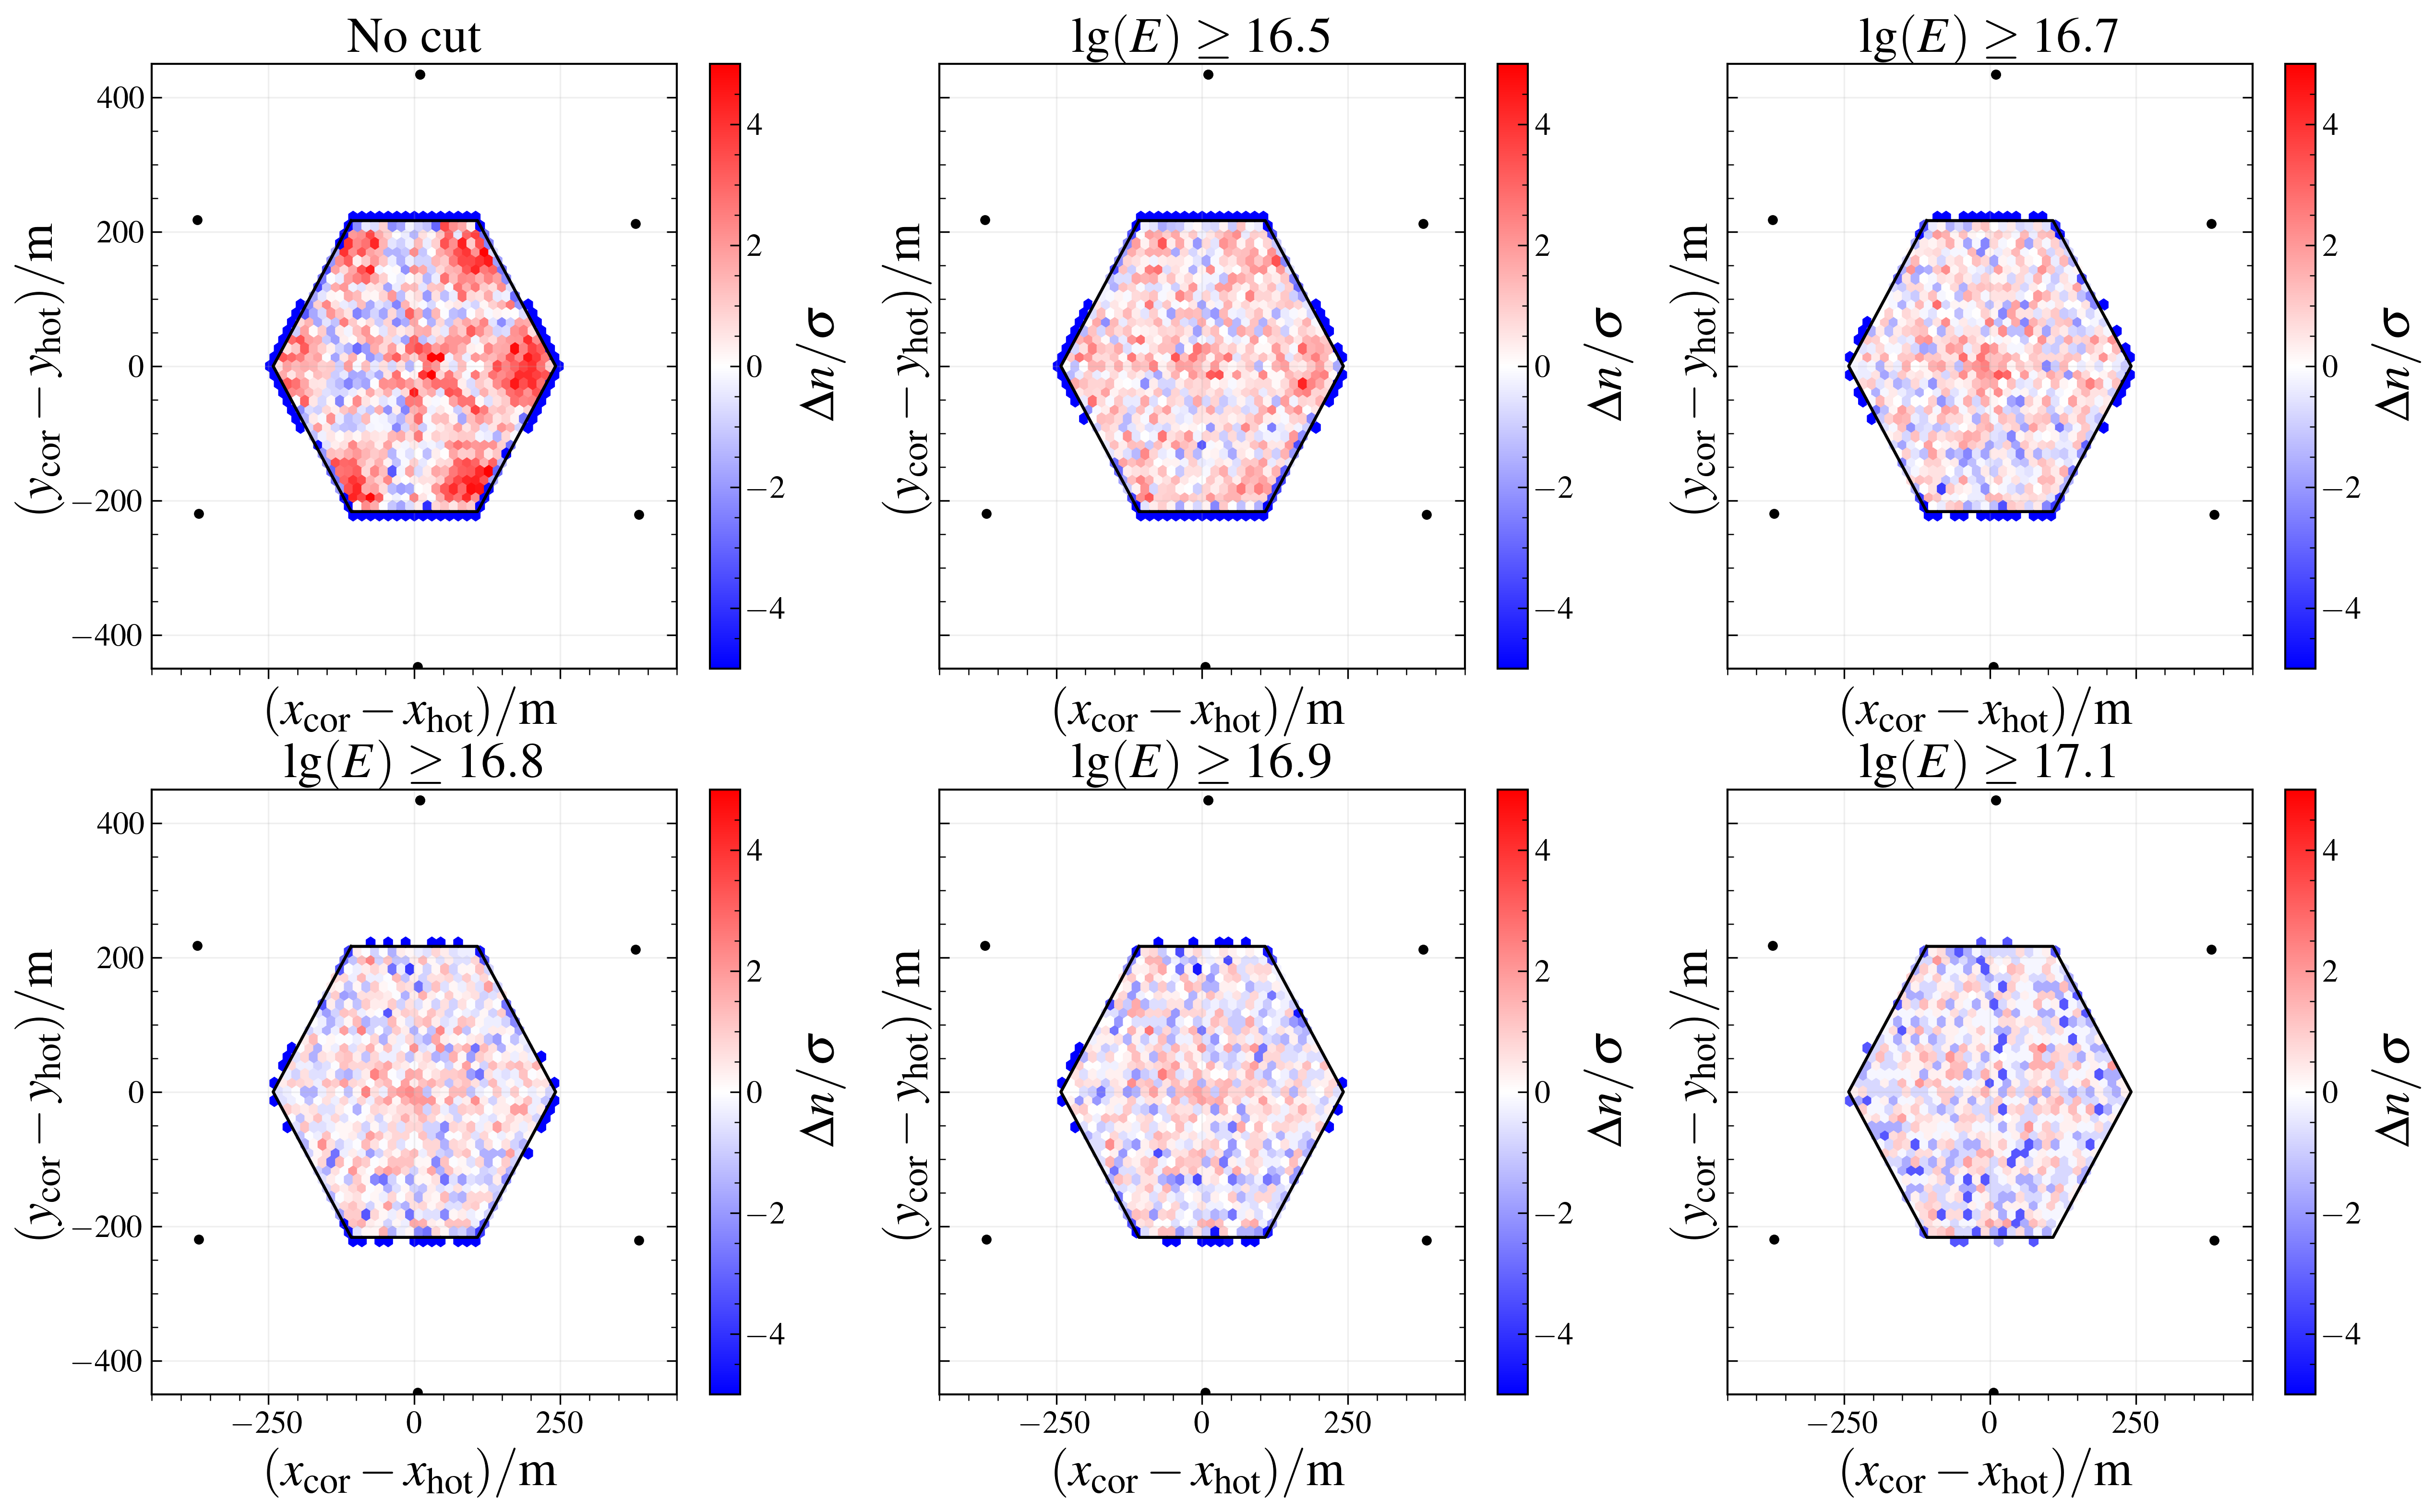
\includegraphics[width=\linewidth]{figures/chapter_dataset/core_distribution_maps.png}
    \caption{Distribution of reconstructed core positions in the fiducial area for different minimum-energy thresholds, using events with $\theta<40^\circ$.
    The outermost bins are excluded to avoid edge effects associated with events reconstructed close to the fiducial boundary.
    At $\lg(E/\mathrm{eV}) = 16.7$, an overdensity is still visible around the central station, consistent with the reconstruction pulling the core toward the hottest station.
    From $\lg(E/\mathrm{eV}) = 16.8$ onward, the distribution becomes more uniform.}
    \label{fig:sd433_core_maps}
\end{figure}

To quantify the uniformity of the core distribution, the observed bin occupancies were compared with a uniform expectation using the Poisson deviance.
For a sample containing $N$ events distributed among $N_{\mathrm{bin}}$ accepted bins, the expected occupancy under the uniform hypothesis is,
\begin{align}
    \nu=\frac{N}{N_{\mathrm{bin}}}.
\end{align}
The Poisson deviance is then
\begin{align}
    D^2 = 2\sum_i
    \left[
        \nu-n_i+n_i\ln\left(\frac{n_i}{\nu}\right)
    \right],
    \label{eq:poisson_deviance}
\end{align}
where $n_i$ is the observed occupancy of bin $i$.
Since the overall normalization is determined from the data, the number of degrees of freedom is $N_{\mathrm{bin}}-1$.
The reduced deviance, $D^2/\mathrm{dof}$, is used to compare samples selected using different minimum-energy thresholds.

The resulting reduced deviance, $D^2/\mathrm{dof}$, is shown in \cref{fig:sd433_core_deviance}.
It decreases as the minimum-energy threshold increases and falls below unity at $\lg(E_{\min}/\mathrm{eV})=16.8$.
This result supports the use of $\lg(E/\mathrm{eV})=16.8$ as the lower boundary of the full-efficiency regime for events with $\theta<40^\circ$.


\begin{figure}
    \centering
    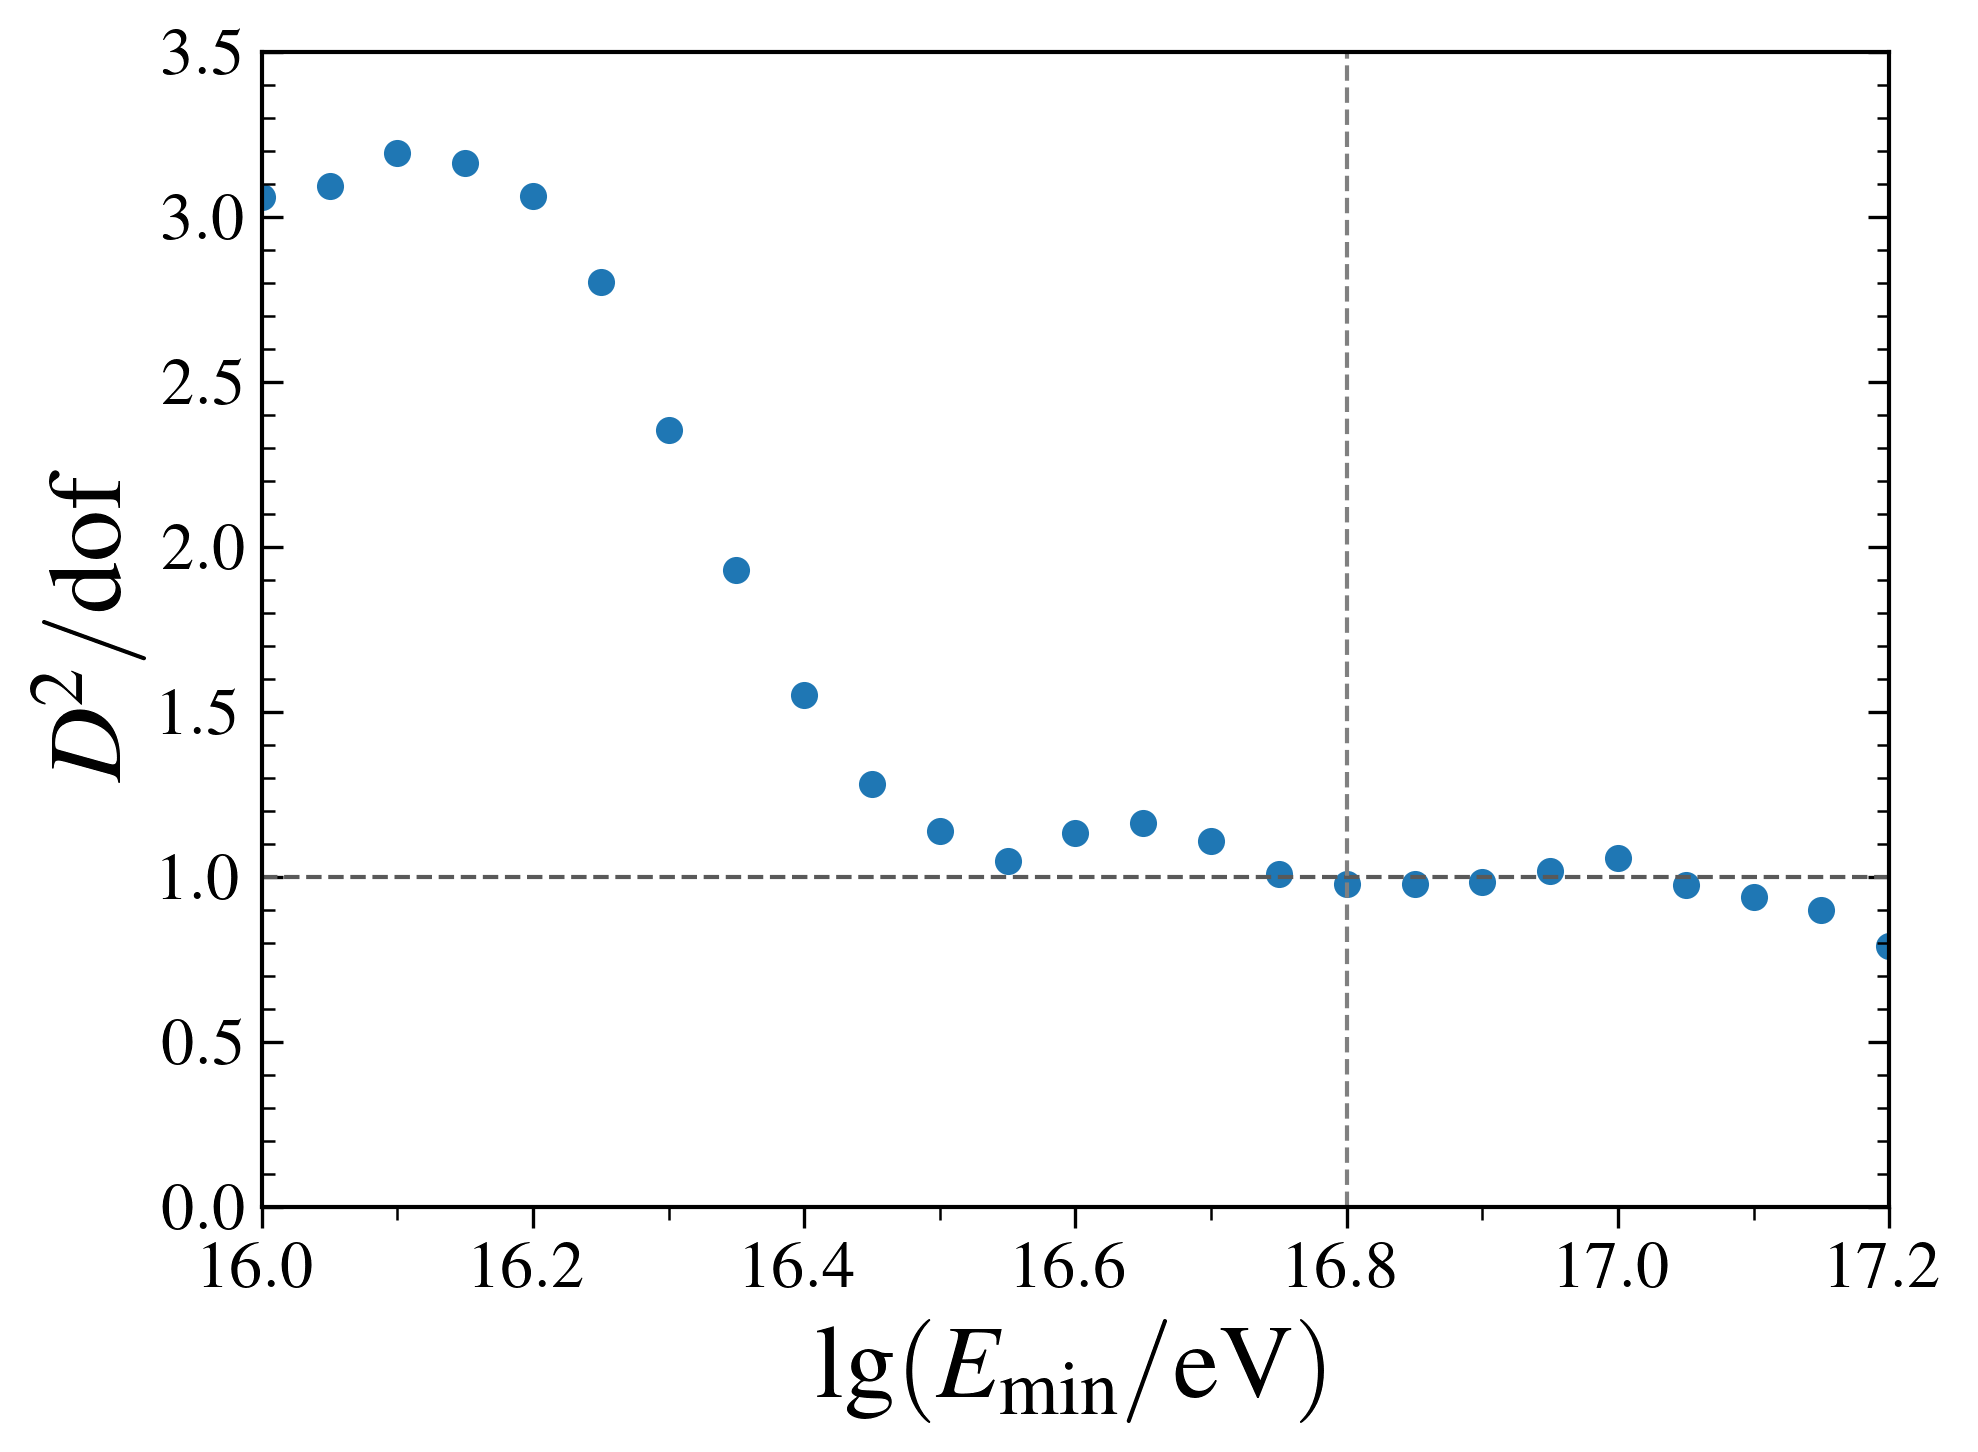
\includegraphics[width=0.75\linewidth]{figures/chapter_dataset/core_distribution_deviance.png}
    \caption{Reduced Poisson deviance of the reconstructed core distribution with respect to a uniform expectation as a function of the minimum-energy threshold, for events with $\theta<40^\circ$.
    The reduced deviance falls below unity at $\lg(E_{\min}/\mathrm{eV})=16.8$, supporting the adoption of this value as the beginning of the full-efficiency regime.
    Its increase at the highest thresholds is associated with the larger statistical fluctuations caused by the lower bin occupancies.}
    \label{fig:sd433_core_deviance}
\end{figure}

The simulation-based efficiency determination and the two data-driven validations therefore support the adoption of $\lg(E/\mathrm{eV})=16.8$, corresponding to $\SI{0.063}{\exa\eV}$, as the full-efficiency threshold for the \sd{433} dataset.
Above this threshold, the exposure can be calculated from the geometric aperture of the array given that the efficiency factor in this calculation is unity


%%%%%%%%%%%%%%%%%%%%%%%%%%%%%%%%%%%%%%%%%%%%%%%%%%%%%%%%%%%%%%%%%%%%%%%%%%%
\section{Array stability}
\label{sec:stability}
%%%%%%%%%%%%%%%%%%%%%%%%%%%%%%%%%%%%%%%%%%%%%%%%%%%%%%%%%%%%%%%%%%%%%%%%%%%

The \sd{433} evolved from an engineering array around the Tina Turner station into its seven-hexagon configuration over a six-year period.
During this time, changes to the detector layout and communication system affected both the number of active stations and the information available to evaluate the 6T5 condition.

The main stages relevant to the dataset used in this work are summarized below~\cite{GAP:Roncoroni:2021:Recovery}:
\begin{itemize}
    \item April 2013: stable data acquisition began with a single hexagon.
    \item January 2014: the \gls{totd} and \gls{mops} triggers were deployed.
    \item June--December 2017: the stations Chichino Jr. and Guili Jr. were repositioned.
    \item January 2018: the array was expanded to four hexagons.
    \item July 2018: silent stations were included in the acquired events.
    \item May 2019: installation of the seven-hexagon configuration was completed.
    \item December 2021: the electronics upgrade for Phase II began.
\end{itemize}

The status of non-triggered stations was not included in the event records in the origina array.
Consequently, the 6T5 trigger could not be evaluated, resulting in a substantial deficit of events satisfying this quality requirement.
Although the earlier data were subsequently recovered using monitoring information~\cite{GAP:Roncoroni:2021:Recovery}, the dataset used in this work begins on 1 July 2018, when silent stations were included in the events.
Restricting the analysis to this period ensures that the 6T5 trigger is evaluated directly from the detector-status information included in the acquired event records and provides a homogeneous dataset throughout the analysis.
The selected period ends on 21 December 2021, when the electronics upgrade of the \sd{433} array began.

The stability of the array is monitored using the daily event rate shown in \cref{fig:event_rate}.
\begin{figure}
    \centering
    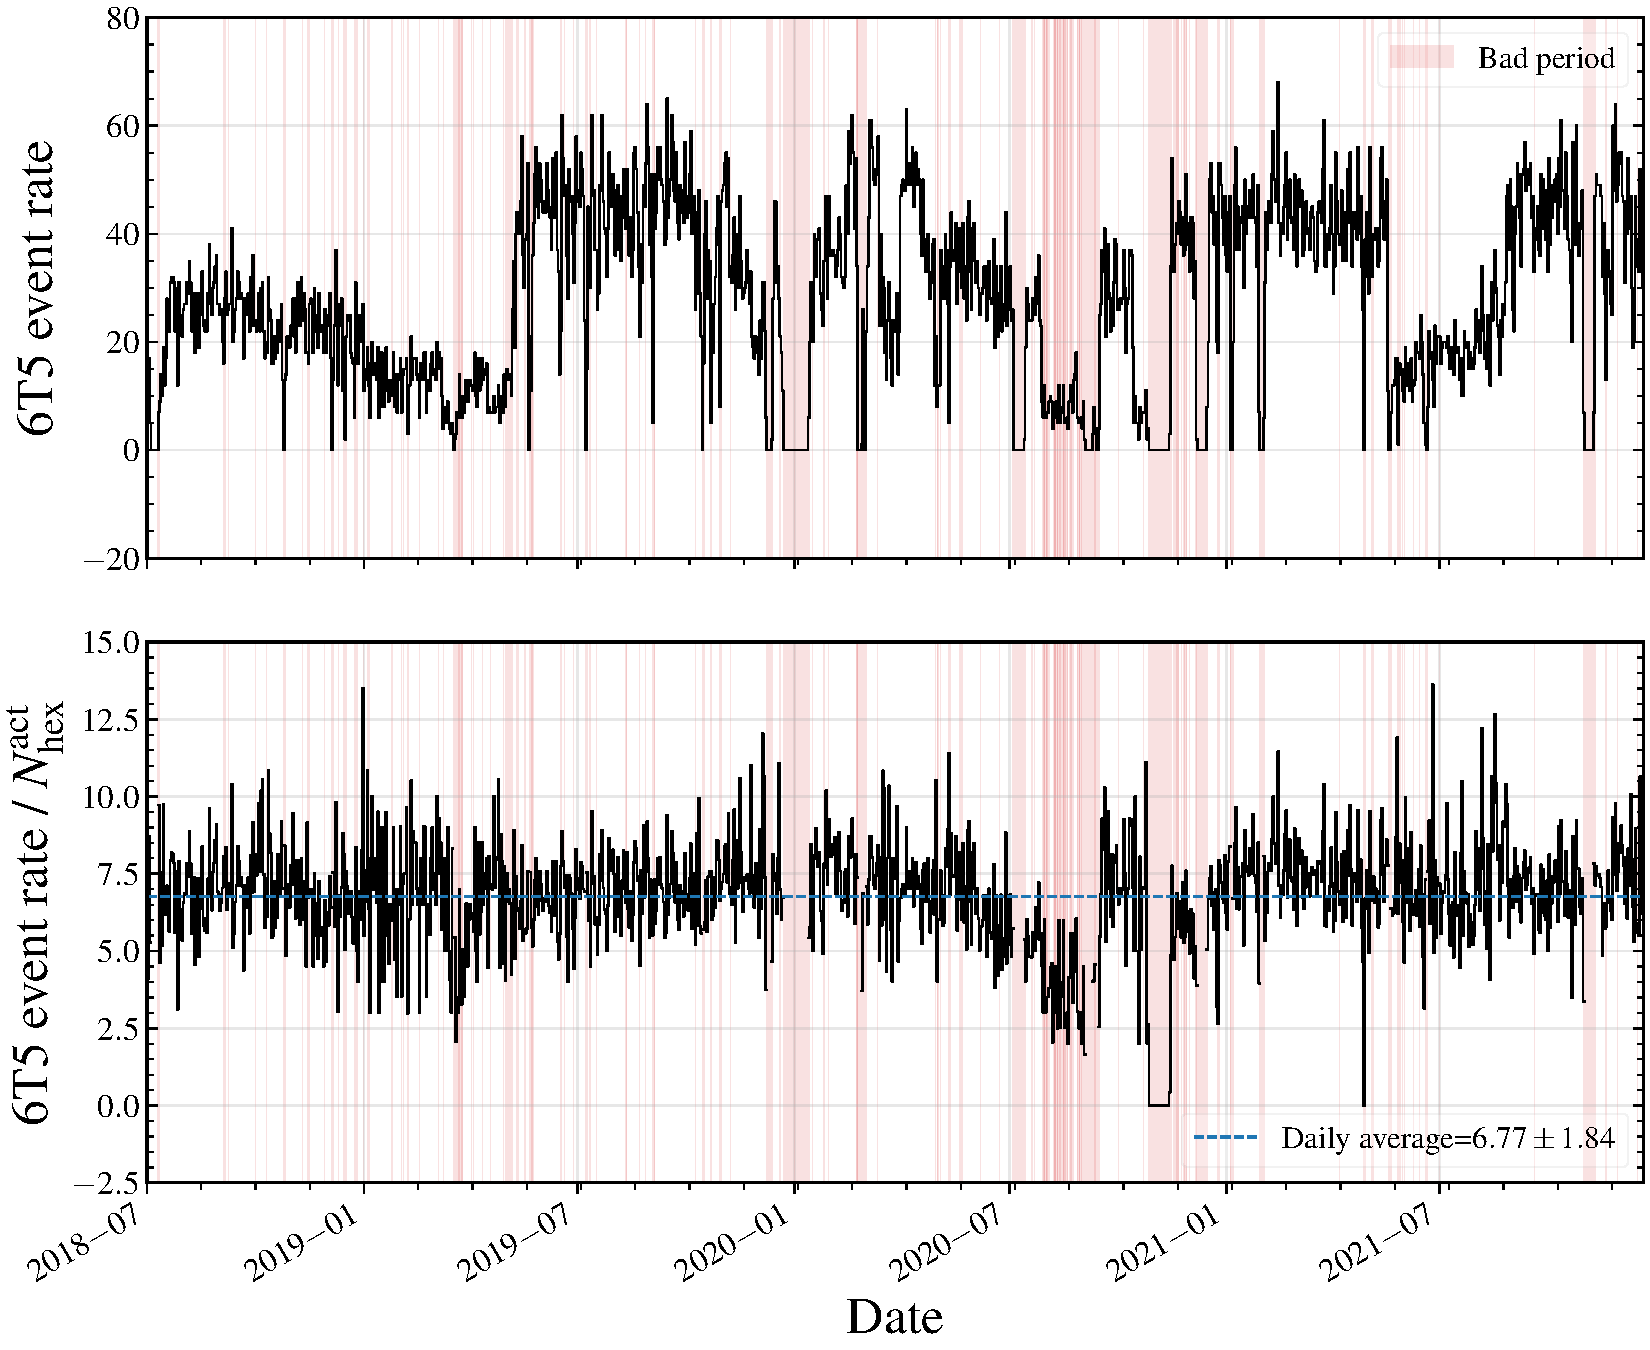
\includegraphics[width=\linewidth]{figures/chapter_dataset/event_rate.pdf}
    \caption{Top: Daily rate of 6T5 events with $\lg(E/\mathrm{eV})>16.8$ during the acquisition period used for the spectrum.
    Bottom: The same event rate normalized by the number of active hexagons calculated from the T2Life information.
    The horizontal line indicates the average normalized event rate, and the shaded regions indicate the periods of unstable acquisition excluded from the  analysis.}
    \label{fig:event_rate}
\end{figure}

The increase in the total event rate observed in 2019 results from the addition of three new hexagons to the array.
To separate changes in the array size from variations in its operational stability, the event rate is normalized by the number of active hexagons at each time, as shown in \cref{fig:event_rate}.
For a stable detector configuration, the normalized rate is expected to remain approximately constant, so significant deviations can be used to identify changes in the acquisition conditions.

The operational status of each station is recorded every second and indicate whether a station is capable of acquiring data in the so-called T2Life flags.
A hexagon is considered active when its central station and all six stations in its first crown are tagged as alive.
The instantaneous array configuration can therefore be evaluated with a time resolution of one second~\cite{GAP:Gonzalez:2022:Exposure}.
% For the exposure calculation, this information is summarized in one-minute intervals, within which the number of active hexagons is treated as constant.
For the selected 1269-day acquisition interval, the daily rate is calculated using 6T5 events with $\lg(E/\mathrm{eV})>16.8$, without applying the zenith-angle selection.
After normalization by the number of active hexagons, the rate has a mean of $6.8$ events per day per hexagon and a standard deviation of $\sigma_{N_{\mathrm{evt}}}=1.8$.

Although the surface detector has a duty cycle close to $100\%$, communication and electronics failures can produce periods of unstable data acquisition.
These periods are identified from unexpectedly long time intervals between successive 6T5 events.
%Assuming that the events follow a Poisson process, their expected rate is proportional to the active area.
The probability of observing a time interval longer than $T$ is,
\begin{align}
    P(t>T)=\exp(-F\,A \,T),
\end{align}
where $F$ is the expected event rate per unit time and unit area and $A$ is the average effective area of the active hexagons during the interval.
An interval is classified as unstable when this probability falls below a threshold set to $\alpha=10^{-2.5}$~\cite{GAP:Gonzalez:2022:Exposure}.
The intervals satisfying $P(t>T)<\alpha$, referred to as \textit{bad periods}, are shaded in \cref{fig:event_rate}.
Together, these bad periods account for $170$ days of the $1269$-day acquisition interval, corresponding to an exposure loss of about $13\%$.

% However, in December 2017, it was noticed that the positions of two of the stations of the first crown, Chichino and Guili, were  35 and 75\,m away from the expected position respectively.
% These stations were then relocated to correct their positions.
% To study the stability of the array, we will use events detected in coincidence with \sd{750}, that will be used for the energy calibration as will be explainded in \cref{chap:energy_calibration}.
% \Cref{fig:time_stability} shows the average energy bias from \sd{433} and \sd{750} as a function of time, together with the daily average.
% It can be seen that there is a difference in the trend of the bias for events before and after Dec. 2017.
% This coincides with the relocation of first Chichino and then Guili.
% For this reason, events before Jan. 2018 weren't considered in the spectrum presented at ICRC 2023.

%%%%%%%%%%%%%%%%%%%%%%%%%%%%%%%%%%%%%%%%%%%%%%%%%%%%%%%%%%%%%%%%%%%%%%%%%%%
\section{Exposure of the \sd{433}}
\label{sec:exposure}
%%%%%%%%%%%%%%%%%%%%%%%%%%%%%%%%%%%%%%%%%%%%%%%%%%%%%%%%%%%%%%%%%%%%%%%%%%%

After establishing the full-efficiency threshold and identifying the periods of stable acquisition, the exposure can be determined geometrically.
% Above the full-efficiency threshold, the detection probability can be considered independent of the primary energy and mass, and the detector aperture is obtained by integrating its effective projected area over solid angle.
The fiducial area associated with one active 6T5 hexagon is given by \cref{eq:6T5_area}.
Acceptance describes the ability of the array to collect particles from different directions. For a flat collecting surface, the area seen from an arrival direction is its projected area, \(S_{\mathrm{hex}}\cos\theta\).
The acceptance of an elemental hexagon in a acceptance cone  delimited by the zenith angles $\theta_{\min}$ and $\theta_{\max}$ is found by integration that projected area over all accepted directions,

\begin{align}
    A_{\mathrm{6T5}}
    &=S_{\mathrm{hex}}
    \int_0^{2\pi}\mathrm{d}\phi
    \int_{\theta_{\min}}^{\theta_{\max}}
    \cos\theta\sin\theta\,\mathrm{d}\theta \\
    &=\frac{\sqrt{3}}{2}d^2\pi
    \left(
        \sin^2\theta_{\max}
        -\sin^2\theta_{\min}
    \right).
\end{align}
\noindent For the zenith-angle range used in this work, $\theta_{\min}=0^\circ$ and $\theta_{\max}=40^\circ$, the acceptance per active hexagon is $A_{\mathrm{6T5}}=\SI{0.211}{\km\squared\sr}$.
The acceptance for the array containing $N_{\mathrm{hex}}$ active hexagons is,
\begin{align}
    \frac{\mathrm{d}\exposuresym}{\mathrm{d}t}
    =N_{\mathrm{hex}}(t)A_{\mathrm{6T5}}.
\end{align}
The accumulated exposure is obtained by integrating this acceptance over the selected acquisition intervals,
\begin{align}
    \exposuresym
    =\int_{\mathrm{good\ periods}}
    N_{\mathrm{hex}}(t) \, A_{\mathrm{6T5}}  \,\mathrm{d}t,
\end{align}
\indent where the identified bad periods are excluded.
% In this way, stable periods with a reduced number of active hexagons are retained, with their contribution weighted by the corresponding instantaneous aperture.

The upper panel of \cref{fig:exposure} shows the daily mean number of active hexagons calculated from the minute-based T2Life information.
Its evolution reflects both changes in the array configuration and temporary detector downtime.
Their maximum corresponds to all 7 hexagons of the \sd{433} in good working order.
The lower panel shows the accumulated exposure contributed by each hexagon and their sum after excluding the bad-acquisition periods.

The total accumulated exposure for $\theta<40^\circ$ is \SDFourThreeThreeExposure.
\begin{figure}
    \centering
    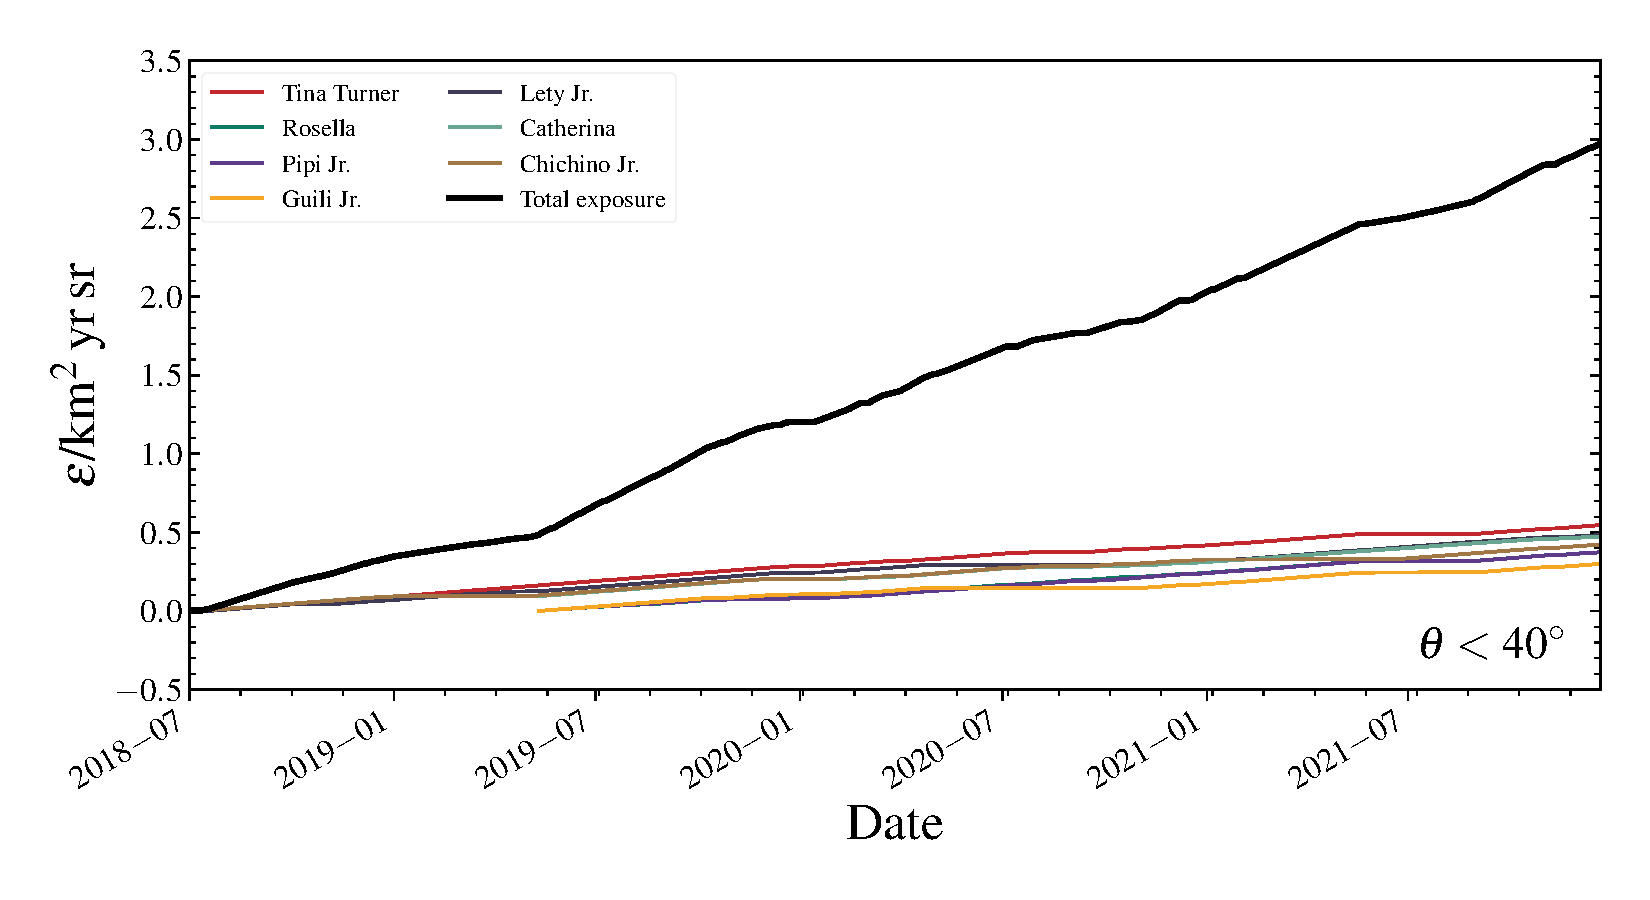
\includegraphics[width=\linewidth]{figures/chapter_dataset/acumulated_exposure.pdf}
    \caption{Evolution of the \sd{433} array and its exposure during the selected data period.
    Top: daily mean number of active 6T5 hexagons calculated from the T2Life information.
    Bottom: accumulated exposure of the individual hexagons and their sum for $\theta<40^\circ$ after excluding bad-acquisition periods.}
    \label{fig:exposure}
\end{figure}

Applying the 6T5 quality condition, the full-efficiency threshold $\lg(E/\mathrm{eV})\geq16.8$, and the zenith-angle selection $\theta<40^\circ$ yields \SDFourThreeThreeNEvents events.

\section{Chapter summary}
\label{sec:sd433_dataset_summary}

This chapter presented the trigger, efficiency, and stability requirements used to define the \sd{433} dataset for the measurement of the cosmic-ray energy spectrum.
The hierarchical trigger system identifies physical air-shower events, while the 6T5 quality condition selects showers whose cores lie within an active region of the array and can therefore be reliably reconstructed.

The detector efficiency was determined using simulations and validated with measured data through the distributions of the arrival directions and reconstructed shower cores.
These studies support the choice of $\lg(E/\mathrm{eV})=16.8$ as the lower boundary of the full-efficiency regime for events with $\theta<40^\circ$.
Above this threshold, the aperture can be calculated geometrically because the detection probability can be considered independent of the primary energy and mass.

The operational history and active configuration of the array were characterized using the T2Life information.
Periods of unstable acquisition were identified and excluded, while the number of active 6T5 hexagons was used to integrate the time-dependent acceptance.
The final dataset covers the period from 1 July 2018 to 21 December 2021 and has a live-time fraction of $87\%$.
After applying the 6T5 quality condition, the full-efficiency threshold, and the zenith-angle selection, it contains \SDFourThreeThreeNEvents events with an accumulated exposure of \SDFourThreeThreeExposure.
This dataset is used in the following chapter to determine the \sd{433} cosmic-ray energy spectrum.

\end{document}
